\documentclass[10pt,a4paper]{article}
\usepackage{amsmath}
\usepackage{ctex}
\usepackage{graphicx}

\title{第四章 流体}
\author{华中科技大学大学物理A}
\date{\today}
\begin{document}
\maketitle
\section{notes}
\subsection{理想流体的运动}
def理想流体:绝对不可压缩($\rho$为常量),无粘性.

稳定流动、欧拉法、流速场、流线、流管.

体积流量$Q=Sv$

由质量守恒得连续性方程
\[\rho_1\Delta S_1v_1=\rho_2\Delta S_2v_2\]
\\理想流体$\rho=constant$,则
\[\Delta Sv=constant\]
\\对分支流管,中间隔开看作两个流管,有
\[\Delta Sv=\Delta S_1v_1+\Delta S_2v_2\]

理想流体的伯努利方程
\[\boxed{p+\rho gh+\frac{1}{2}\rho v^2=constant}\]
连续性方程+功能原理推导
\\其中$p$和$\rho gh$是静压强,$\frac{1}{2}\rho v^2$是动压强.
\\分支流管的伯努利方程:
\[p+\rho gh+\frac{1}{2}\rho v^2=p_1+\rho gh_1+\frac{1}{2}\rho v_1^2\]
\[p+\rho gh+\frac{1}{2}\rho v^2=p_2+\rho gh_2+\frac{1}{2}\rho v_2^2\]

伯努利方程的应用:空吸、小孔流速($v=\sqrt{2gh}$)、比托管(流速计)、流量计、虹吸
\subsection{黏性流体的运动}
黏性流体因切向的黏性力(内摩擦力)而层流

速度梯度velocity gradient$\frac{dv}{dx}$(相距$dx$的两个流层速度差为$dv$)

\textbf{\textit{Newton viscosity law}}
\[\boxed{F=\eta \frac{dv}{dx}S}\]
$\eta$:coefficient of viscosity($Pa\cdot s$)
$S$为$F$分布的面积
\[\Rightarrow \text{切应力}\tau=\eta \frac{dv}{dx}\]

当流速增大到一定程度时,流层破坏,形成涡流或湍流(turbulent flow)

\textbf{\textit{Reynold number}}
\[\boxed{Re=\frac{\rho vr}{\eta}}\]
是一个纯数,判别黏性流体状态的唯一参数,$Re<1000$层流,$Re>1500$湍流,$1000<Re<1500$过渡流

黏性流体的伯努利方程
\[\boxed{p_1+\rho gh_1+\frac{1}{2}\rho v_1^2=p_2+\rho gh_2+\frac{1}{2}\rho v_2^2+w}\]
其中$w$为单位体积流体损耗的机械能.

\begin{footnotesize}
Example:黏性流体在均匀水平圆管中:
\begin{figure}[h]
\begin{center}
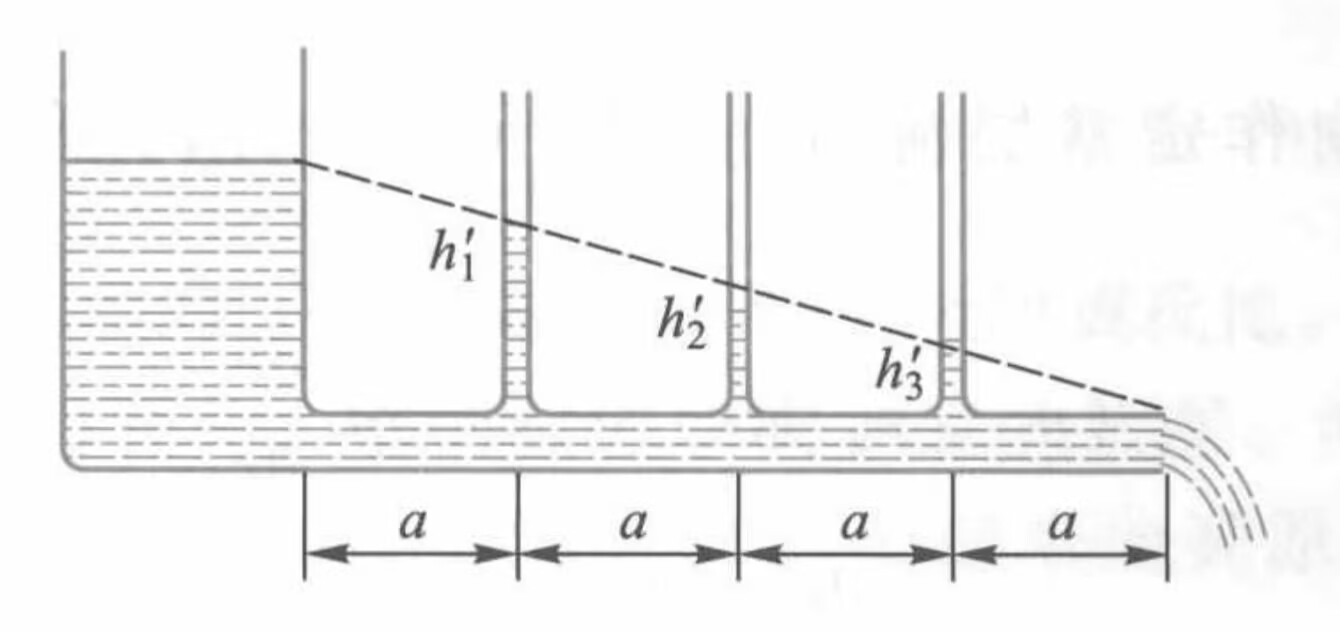
\includegraphics[width=0.5\textwidth]{p1.jpg}
\end{center}
\end{figure}    

粘滞力做功与管长成正比:
\[w=\alpha l\Rightarrow p_0+\rho gh_0-p_0=\alpha l\Rightarrow \alpha=\frac{\rho gh_0}{l}\]
\[p_0+\rho gh_0=p_0+\rho gy+\alpha x\Rightarrow y=-\frac{\alpha}{\rho g}x+h_0\]
\end{footnotesize}

\textbf{\textit{Poiseuilles' law 泊肃叶定律}}
\[\boxed{Q=\frac{\pi R^4(p_1-p_2)}{8\eta L}}\]
即流量与管子半径和压强梯度成正比\\
速度分布:
\[\boxed{v=\frac{p_1-p_2}{4\eta L}(R^2-r^2)}\]
且$v_{max}=\frac{R^2(p_1-p_2)}{8\eta L}$,$\bar{v}=\frac{1}{2}v_{max}$

流阻
\[R_f=\frac{p_1-p_2}{Q}=\boxed{\frac{8\eta l}{\pi R^4}}\]
流阻可串并联

Stokes law:黏性流体中的固体速度不大或线度很小且$Re<1$时
黏性阻力:\[f=6\pi\eta rv\]以此可求收尾速度或沉降速度,如密里根油滴实验
\end{document}